\documentclass{article}
% Packages
\usepackage{amsmath}
\usepackage{amssymb}
\usepackage{graphicx}
\usepackage{booktabs}
\usepackage{algorithmic}
\usepackage{algorithm}
\usepackage{array}

\title{Assignment 1 - Data Mining for Networks}
\author{Correia Ambre - Jeannes Théo}
\date{January $09^{th}$, 2024}
\begin{document}
    \maketitle


    \section{Assignement 1}

    \subsection{Exercice 1}
    1. The derivative of $f(x) = 2x^4 - 4x^3 + 3x^2 + 4x - 3$ is $f'(x) = 8x^3 - 12x^2 + 6x + 4$. \\
    2. The algorithm to do the gradient descent is with $\alpha = 1/10$ is:\\
    \begin{algorithm}
        \caption{Gradient Descent}\label{alg:algorithm}
        \begin{algorithmic}
            \STATE $x := x_0$
            \WHILE{$|8x^3 - 12x^2 + 6x + 4| > \epsilon$}
            \STATE $x := x - 0.1 * (8x^3 - 12x^2 + 6x + 4)$
            \ENDWHILE
            \RETURN $x$
        \end{algorithmic}
    \end{algorithm} \\
    3. If we apply the algorithm starting from 0, we get to $-0.4$ first and end at $-0.317$. If we do the same algorithm starting from 10, we get $-676.4$ and then $248120326.787$. \\
    4. The first gradient descend algorithm seems to converge to the minimum of the function, while the second one is clearly diverging. The learning rate is probably too high, and would need to be decreased to get optimal results.

    \subsection{Exercice 2}


    \section{Assignement 2}

    \subsection{Exercice 1}

    \subsection{Exercice 2}

    The table describing features values for the ideal graph kernel is :

    \begin{table}
        \centering
        \begin{tabular}{|>{\centering\arraybackslash}m{1.5cm}|>{\centering\arraybackslash}m{1cm}|>{\centering\arraybackslash}m{1cm}|>{\centering\arraybackslash}m{1cm}|>{\centering\arraybackslash}m{1cm}|}

            \toprule
            \textbf{}                                                        & 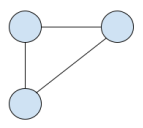
\includegraphics[width=1cm,keepaspectratio]{images/triSujet} & 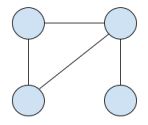
\includegraphics[width=1cm,keepaspectratio]{images/tri+Sujet} & 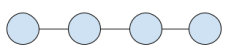
\includegraphics[width=1cm,keepaspectratio]{images/ligneSujet} & 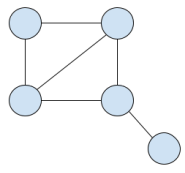
\includegraphics[width=1cm,keepaspectratio]{images/5sujet} \\
            \midrule
            
\includegraphics[width=1cm,keepaspectratio]{images/1}            & 3                                                            & 4                                                             & 4                                                              & 5                                                          \\
            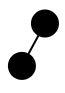
\includegraphics[width=1cm,keepaspectratio]{images/2}            & 3                                                            & 4                                                             & 4                                                              & 6                                                          \\
            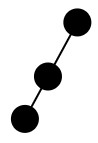
\includegraphics[width=1cm,keepaspectratio]{images/3}            & 3                                                            & 5                                                             & 2                                                              & 9                                                          \\
            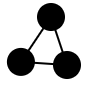
\includegraphics[width=1cm,keepaspectratio]{images/3tr}          & 1                                                            & 1                                                             & 0                                                              & 2                                                          \\
            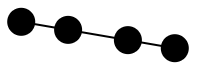
\includegraphics[width=1cm,height=1cm,keepaspectratio]{images/4} & 0                                                            & 1                                                             & 1                                                              & 10                                                         \\
            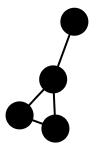
\includegraphics[width=1cm,keepaspectratio]{images/4tr}          & 0                                                            & 1                                                             & 0                                                              & 5                                                          \\
            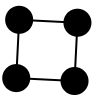
\includegraphics[width=1cm,keepaspectratio]{images/4carre}       & 0                                                            & 0                                                             & 0                                                              & 1                                                          \\
            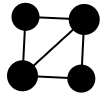
\includegraphics[width=1cm,keepaspectratio]{images/4carBarre}    & 0                                                            & 0                                                             & 0                                                              & 1                                                          \\
            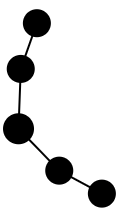
\includegraphics[width=1cm,keepaspectratio]{images/5}            & 0                                                            & 0                                                             & 0                                                              & 4                                                          \\
            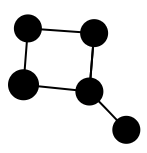
\includegraphics[width=1cm,keepaspectratio]{images/5Carr}        & 0                                                            & 0                                                             & 0                                                              & 1                                                          \\
            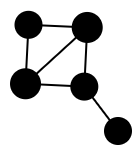
\includegraphics[width=1cm,keepaspectratio]{images/5CarrBare}    & 0                                                            & 0                                                             & 0                                                              & 1                                                          \\
            \bottomrule
        \end{tabular}
        \caption{Feature Values}
    \end{table}

\end{document}
